
\chapter{相关研究综述}
\label{chap:relatedwork}
流行度预测问题自被提出以来,受到了学术界和产业界的广泛关注。本章从流行度的统计特征分析、流行度预测方法以及流行度预测问题的可预测性三个方面入手,对流行度预测领域的相关工作进行了系统的总结和归纳,以便读者更好地了解和掌握该领域的相关知识,进而更好地理解本文的工作。

\section{流行度的统计特征分析}
在线内容的流行度分析工作最早源于网站缓存策略的研究。Cunha等人\citep{chen2005zhulu}在研究站点中网页的访问情况时发现,网页被访问频率的分布服从Zipf定律\citep{chen2005zhulu},也就是说:流行度排名为$i$的网页被用户访问的概率正比于$1/i$,如图\ref{fig:pageDist}所示。这一现象表明,网页的访问频次分布是不均匀的。Almeida等人\citep{chen2005zhulu}在研究万维网中所有网页的访问频次时,也发现了同样的分布规律。
\begin{figure}[!htbp]
  \centering
  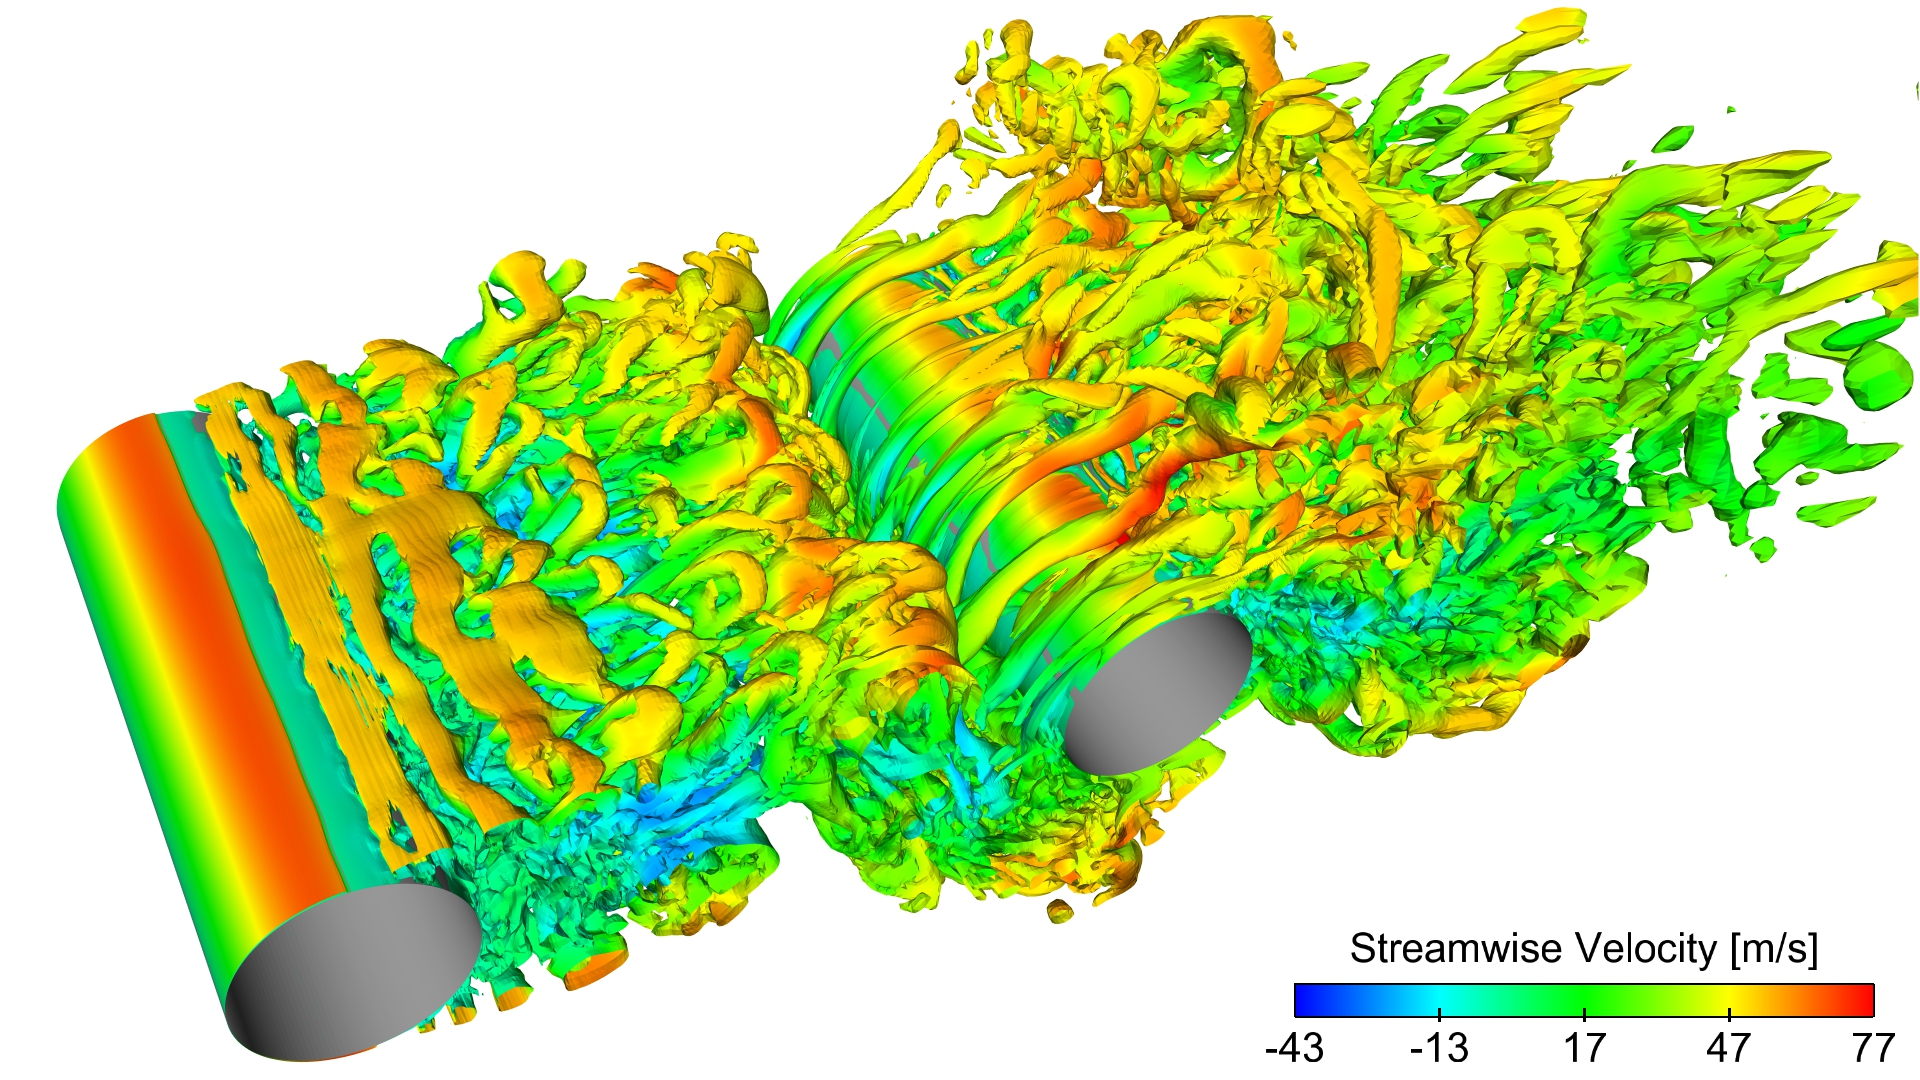
\includegraphics[width=0.45\textwidth]{ITC_Q_Criteria}
  \caption{Q判据等值面图}
  \label{fig:pageDist}
\end{figure}

随着信息技术的发展,视频分享类网站和社交网络平台不断涌现,也引起了研究人员的关注。Gill等人\citep{chen2005zhulu}收集并分析了视频网站Youtube\footnote{\url{https://www.youtube.com}}上视频的访问数据,发现视频的访问频次信息依然服从Zipf定律。Kwak等人\citep{chen2005zhulu}研究了社交网络平台Twitter\footnote{\url{https://twitter.com}}上消息的转发情况,发现参与消息转发的人数服从幂律分布,如图\ref{fig:tweetDist}所示。
\begin{figure}[!htbp]
  \centering
  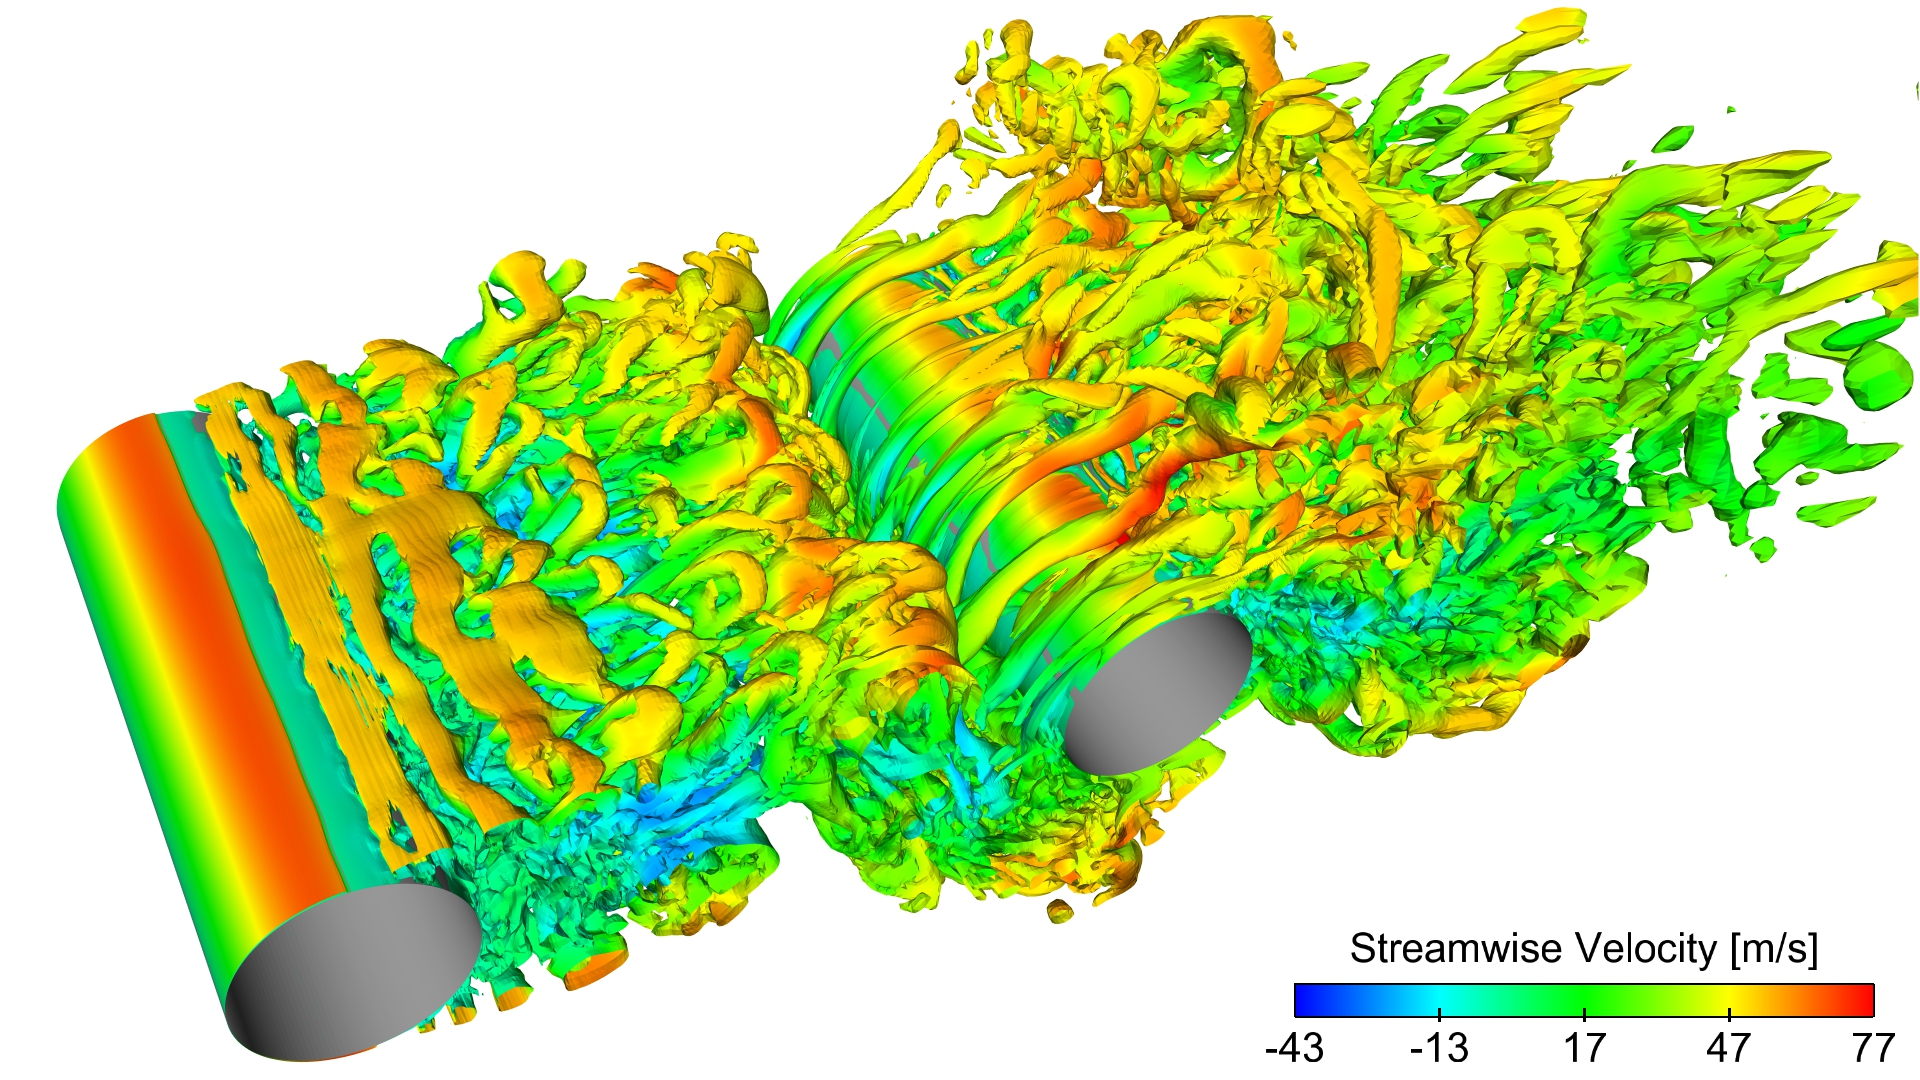
\includegraphics[width=0.45\textwidth]{ITC_Q_Criteria}
  \caption{Q判据等值面图}
  \label{fig:tweetDist}
\end{figure}

除了对宏观的流行度统计量的分析之外,还有一部分工作研究了流行度增长过程中的微观统计特征。Barabasi等人\citep{chen2005zhulu}研究了人类的行为数据,发现人类的行为模式中存在爆发现象:
\section{流行度预测方法概述}
\section{流行度预测问题的可预测性分析}

